\newpage



%\setcounter{section}{1}  
%\setcounter{page}{1}

\section{Project Description}


\subsection{Overview}
\label{Overview}
One of the fundamental challenges in nuclear physics is to understand
why nucleonic matter is stable, how it comes into being, how it
evolves and organizes itself, and what phenomena emerge. The task
facing nuclear theorists is to develop the tools to help answer these
questions by relating the existence and properties of nuclei to the
underlying fundamental forces and degrees of freedom. As experimental
efforts have shifted towards the study of rare
isotopes~\cite{Geesaman:2015fha,NSACdecadal,Balantekin:2014opa}, there
has been an increased urgency to develop reliable \emph{ab initio}
calculations to counter the inherent limitations of ``data-driven''
approaches which rely on experimental data to constrain model
parameters, such as the phenomenological shell model and density
functional theory. For decades \emph{ab initio} progress was slowed by
the lack of a consistent theory for the strong inter-nucleon
interactions, and by the computational demands required to handle the
non-perturbative aspects resulting from the ``hard cores'' and strong
tensor forces found in most interaction models.  For many years, the
only option for controlled calculations was to use quasi-exact methods
such as quantum Monte Carlo (QMC) or no-core shell model (NCSM), which
limited the reach of \emph{ab initio} calculations to light $p$-shell
nuclei. Approximate (but systematically improvable) methods that scale
favorably to larger systems, like coupled cluster (CC) theory and
many-body perturbation theory (MBPT), were largely abandoned in
nuclear physics, despite enjoying tremendous success in quantum
chemistry.


Much has changed in recent years, as advances in chiral effective
field theory (EFT), which provides a systematic framework to construct
consistent two- and three-nucleon
interactions~\cite{vanKolck:1999mw,Epelbaum:2009ve,Epelbaum:2015fb,Machleidt:2011bh,Entem:2003th},
together with the development of powerful renormalization group (RG)
methods to transform interactions to much softer
forms~\cite{Bogner:2010pq,Bogner:2003wn,Bogner:2006vp,Bogner:2006pc},
have led to a resurgence of CC and similar methods, and the
development of new ones such as the in-medium similarity
renormalization group (IMSRG)~\cite{Hergert:2015awm}, pushing the
frontiers of \emph{ab initio} theory well into the medium-mass
region~\cite{Tsukiyama:2011uq,Tsukiyama:2012fk,Bogner:2014tg,Jansen:2014qf,Jansen:2015ngw,Stroberg:2015ymf,Stroberg:2016ung,Soma:2013ys,Soma:2014fu,Soma:2014eu,Hergert:2013ij,Hergert:2014vn,Hergert:2016etg,Wienholtz:2013bh,Hagen:2015ve,jansenprl2016}, see Fig.~\ref{fig:abinitio}. Initial
applications of these methods were limited primarily to ground-state
properties of stable nuclei near shell closures with two-nucleon
forces only. Substantial progress has since been made on including
three-nucleon forces~\cite{Hagen:2007zc,Soma:2013xha,Roth:2012qf,Hergert:2012nb}, targeting excited states and observables besides
energy~\cite{Ekstrom:2014iya,Jansen:2012ey}, and moving into the more
challenging terrain of open-shell and unstable
nuclei~\cite{Tsukiyama:2012fk,Jansen:2014qf,Bogner:2014tg,Stroberg:2015ymf,Stroberg:2016ung,Soma:2013ys,Soma:2012zd,Hergert:2013ij,Gebrerufael:2016xih}. The recent work of Jansen {\em et al} \cite{jansenprl2016} on the structure of $^{78}$Ni and nearby nuclei represents some of the progress which has been made recently in pushing the limits of first principle methods. Remarkably,
progress on the many-body front has been so swift in recent years that
inadequacies of the current-generation chiral two- and three-nucleon
interactions, rather than the many-body calculations themselves, are
the primary obstacles to systematic calculations across the
medium-mass region~\cite{Ekstrom:2015fk,Binder:2014fk}.



\begin{figure}[t!]
\centering
   \begin{subfigure}[t]{.5\textwidth}
   \centering
  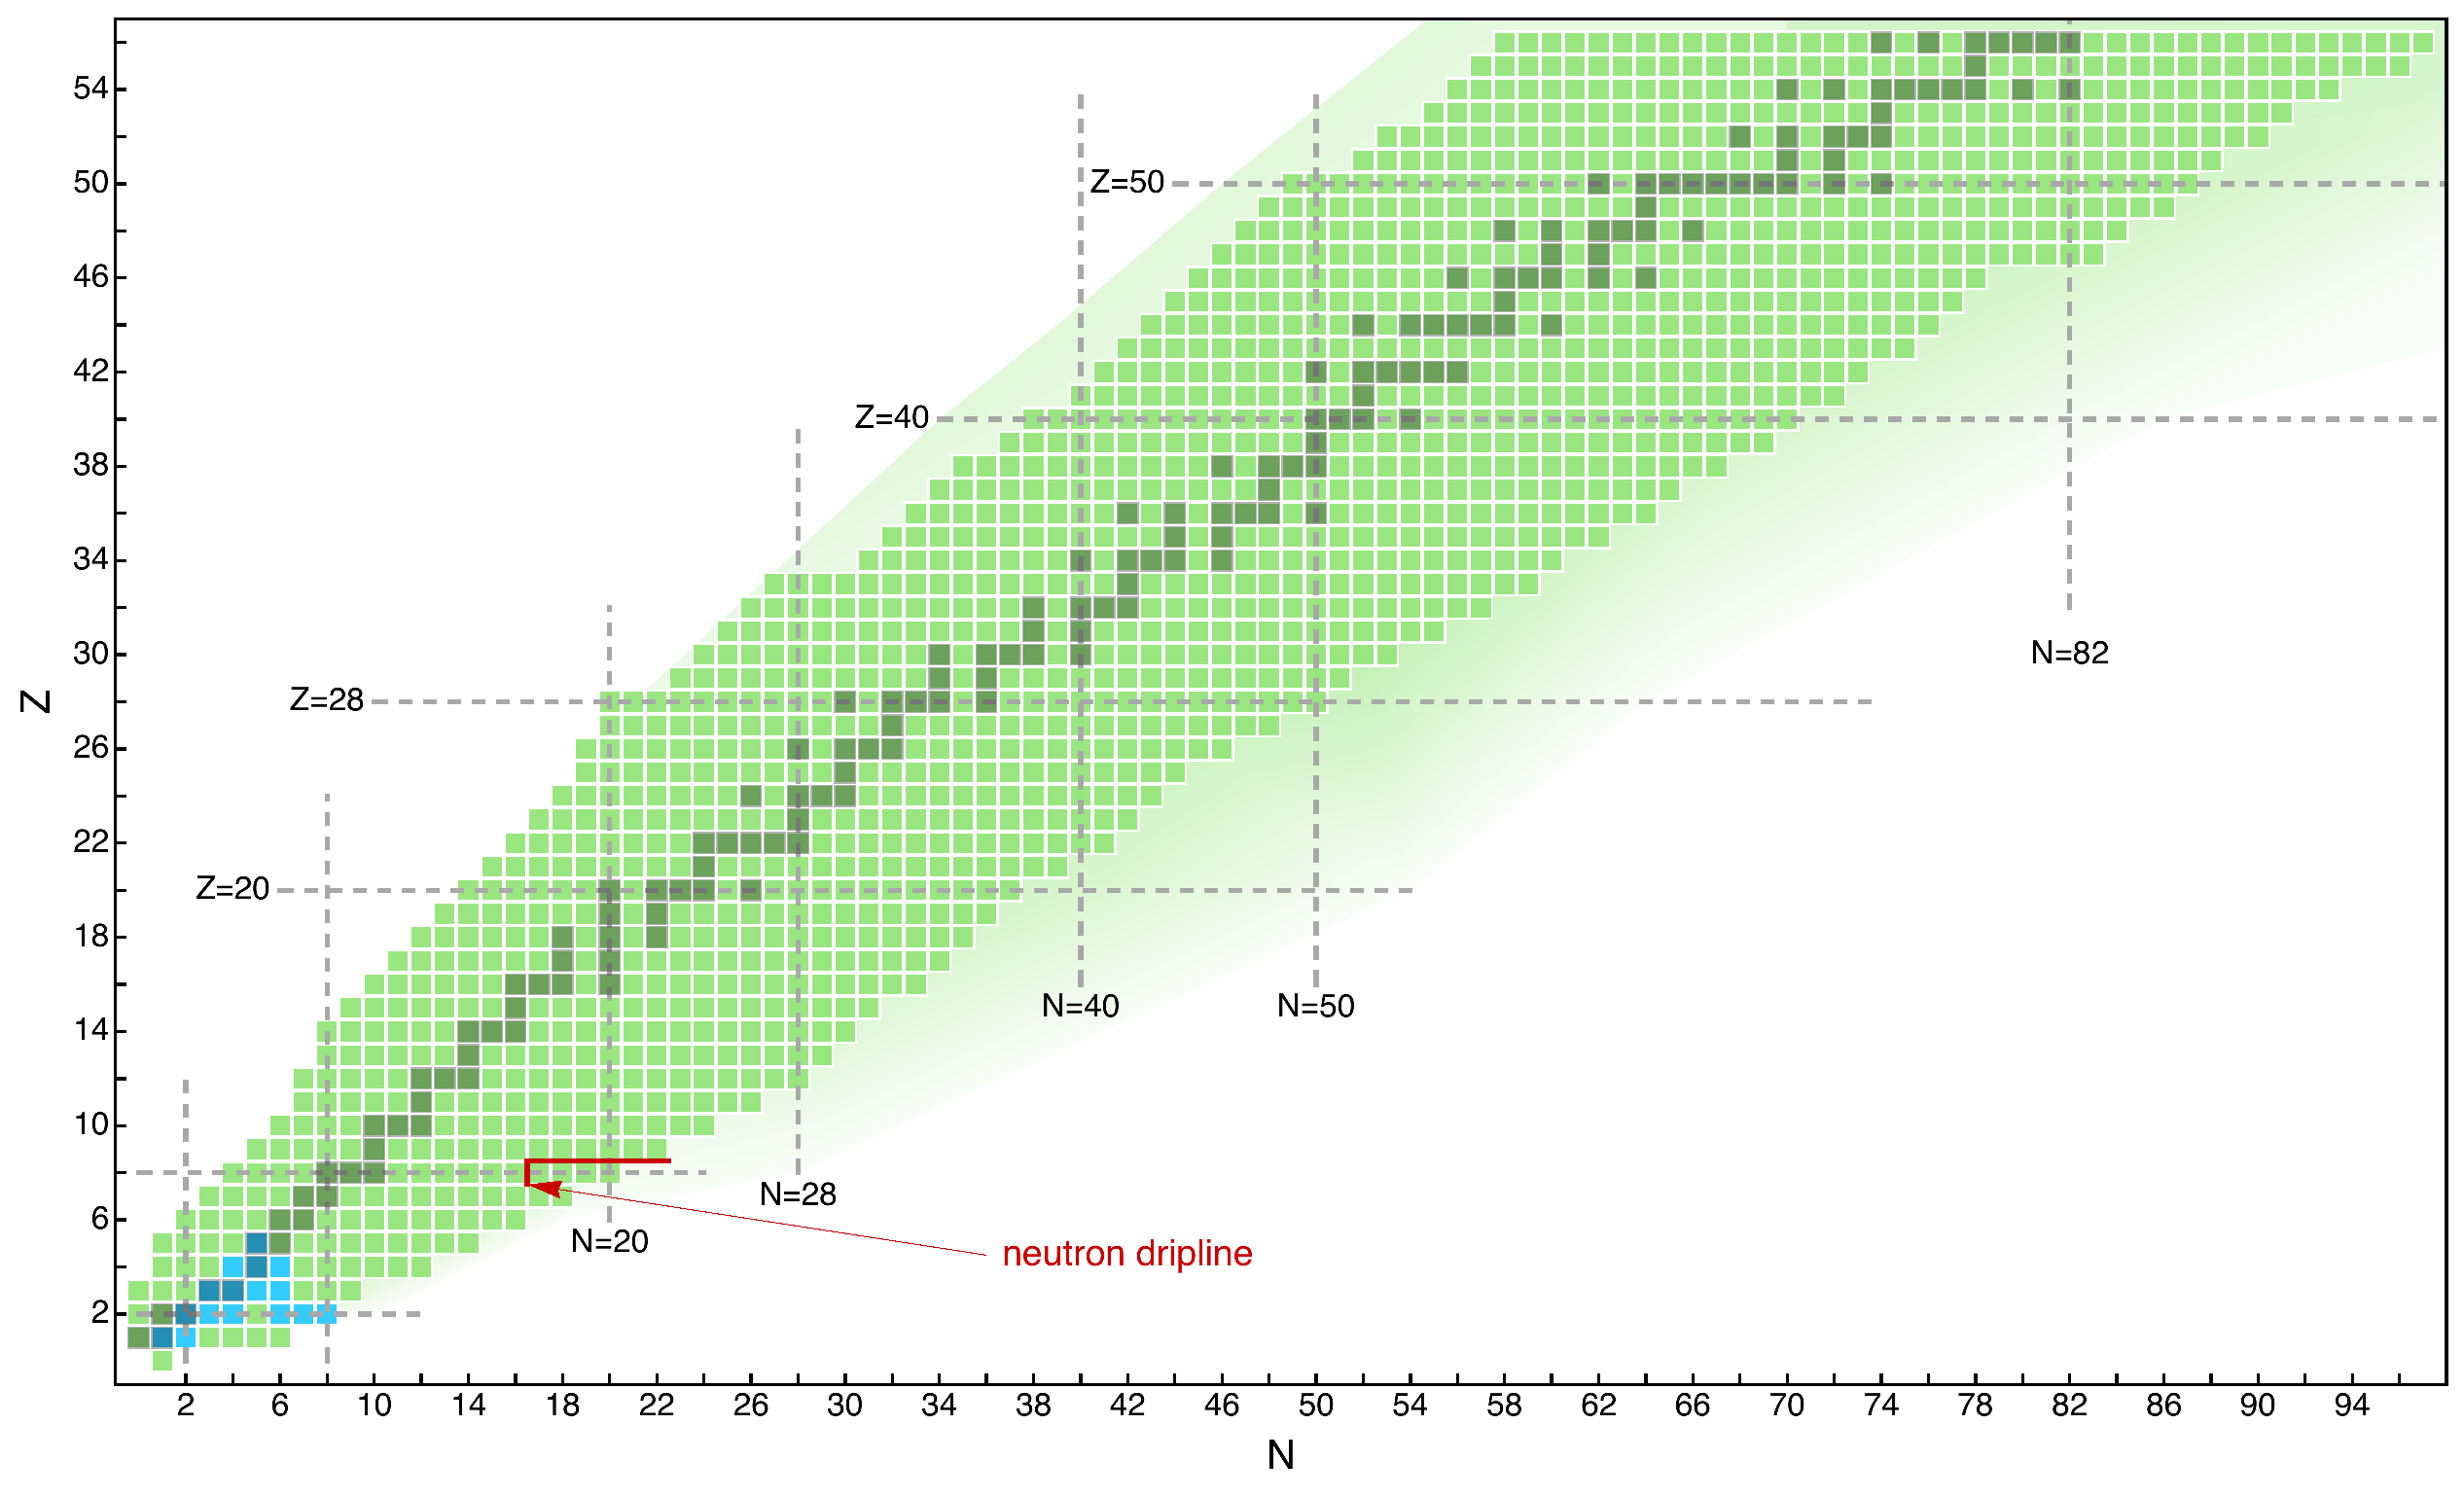
\includegraphics[width=.99\linewidth]{ab-initio_nuclear_chart_2005.eps}
%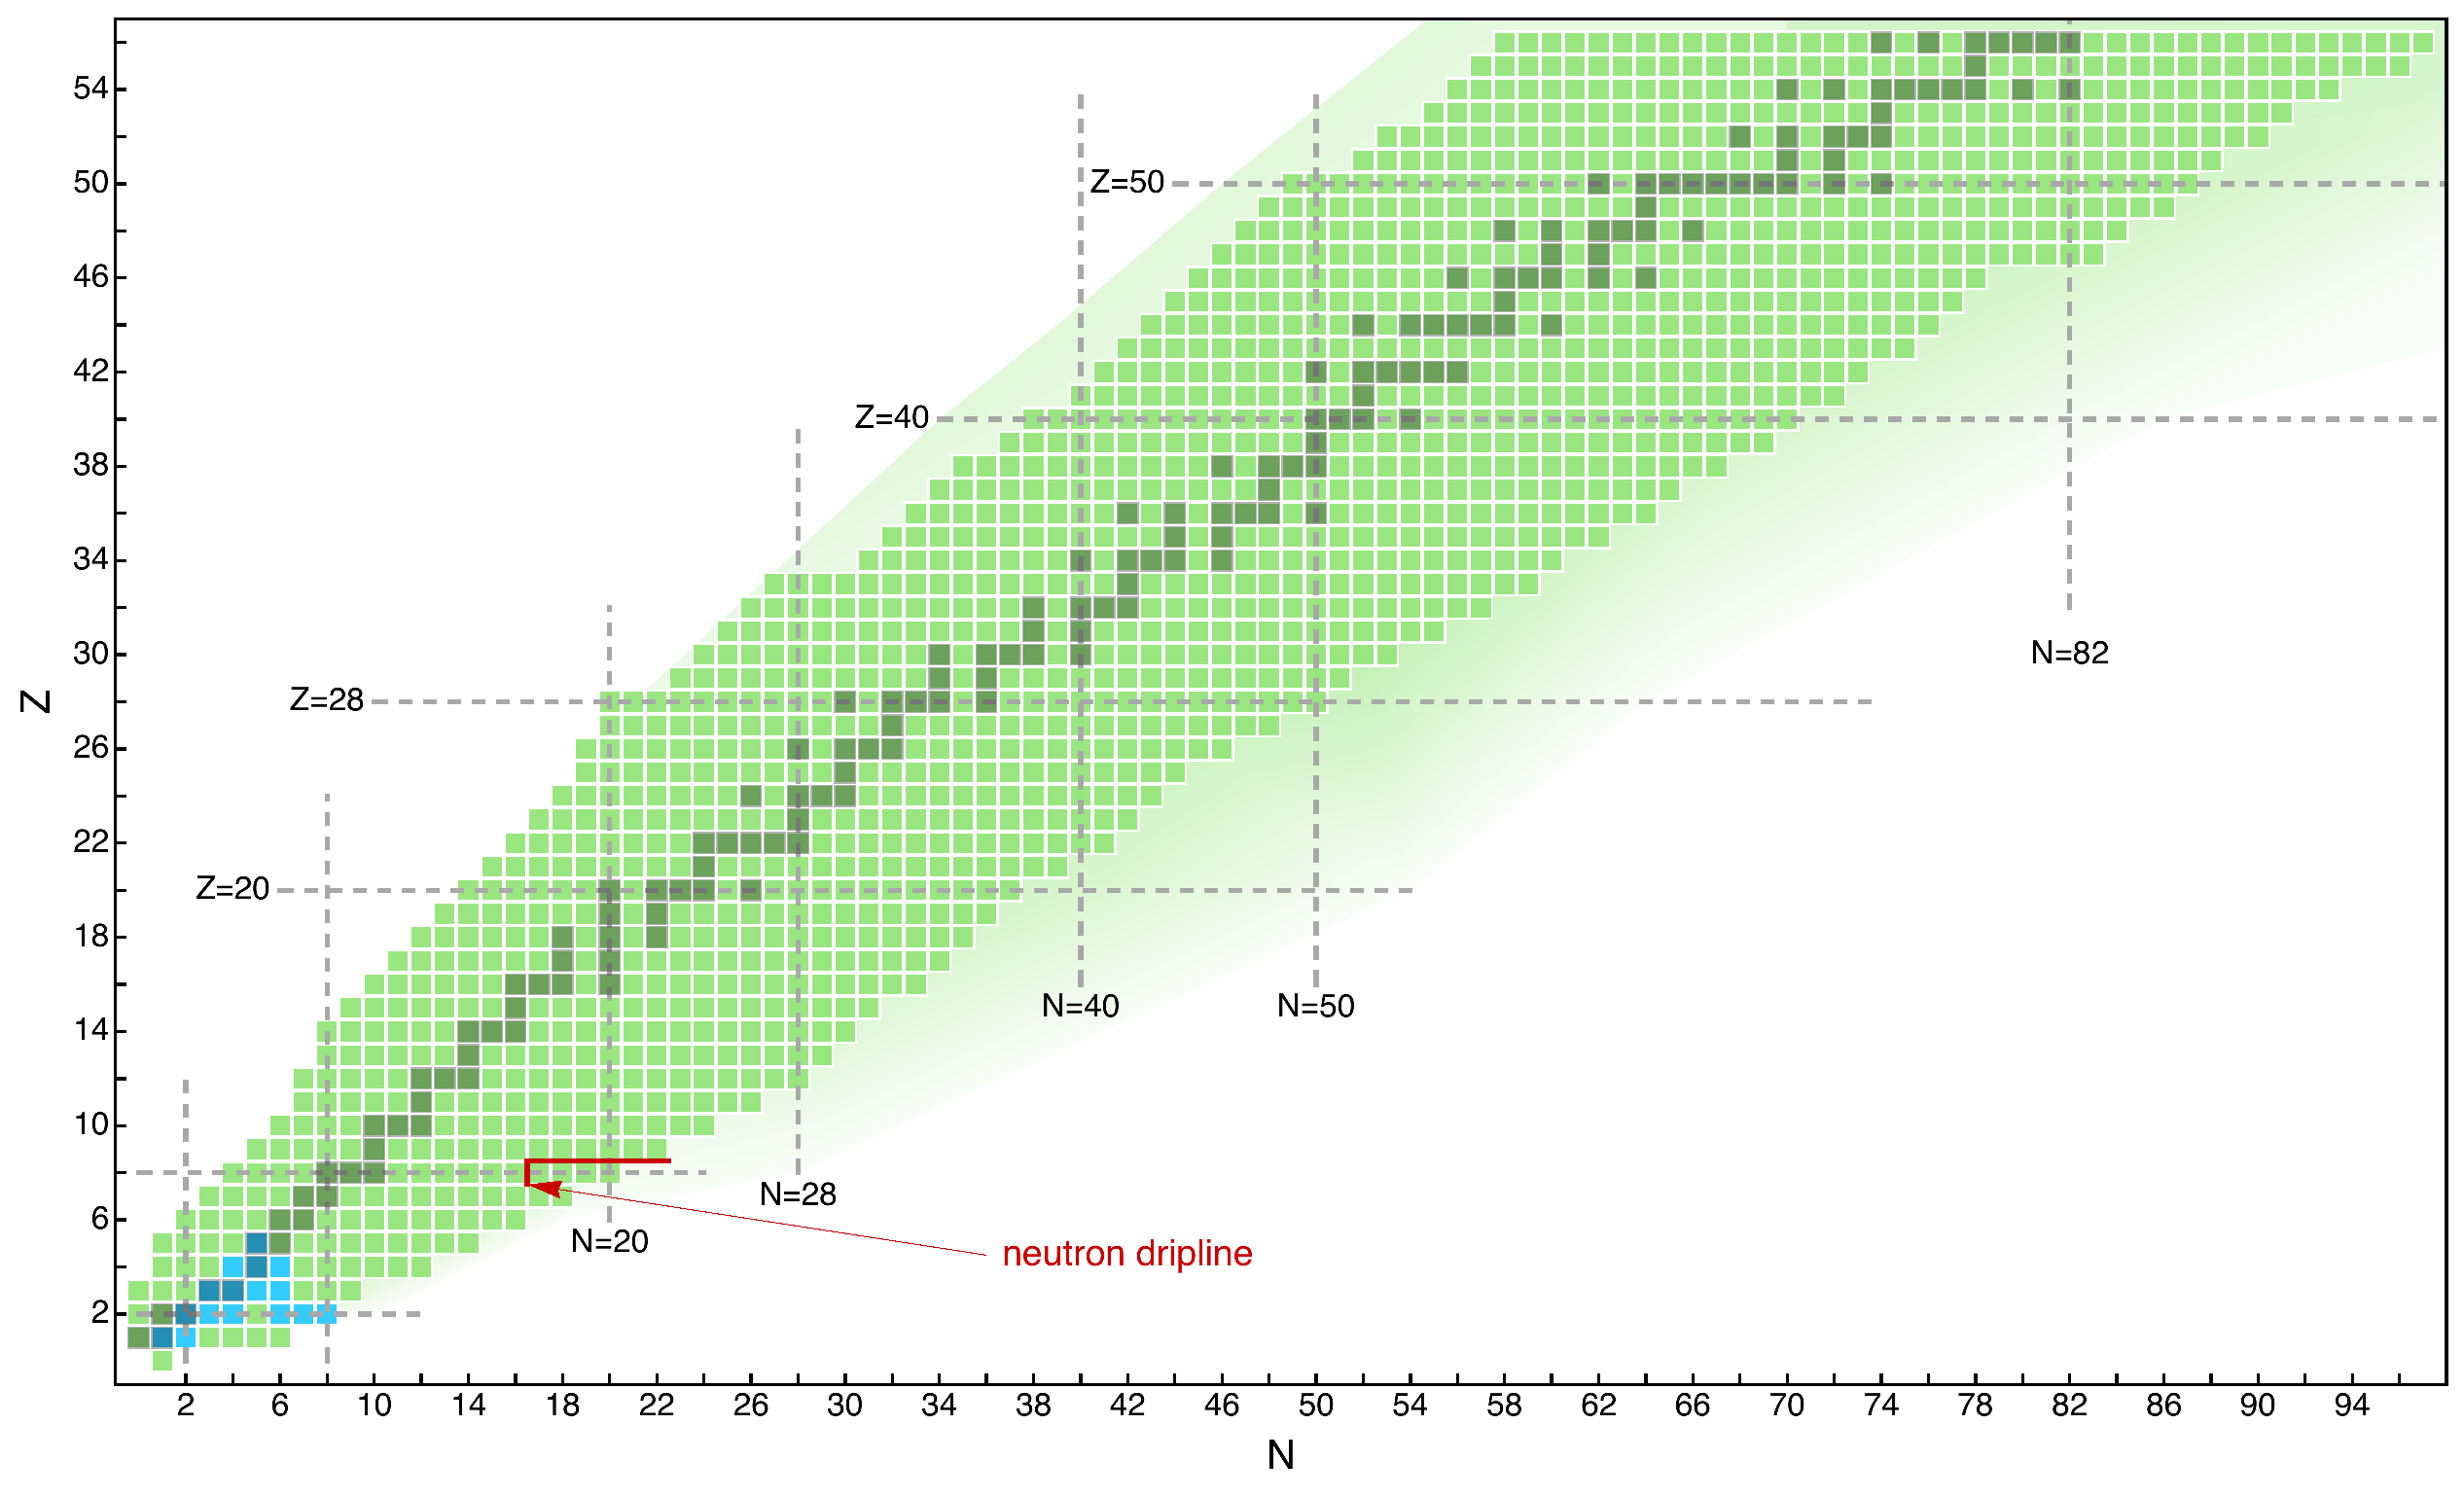
\includegraphics[height=3.0 in]{ab-initio_nuclear_chart_2005.eps}
   \caption{   \label{fig:abinitio2005} }
\end{subfigure}%
\begin{subfigure}[t]{.5\textwidth}
\centering
  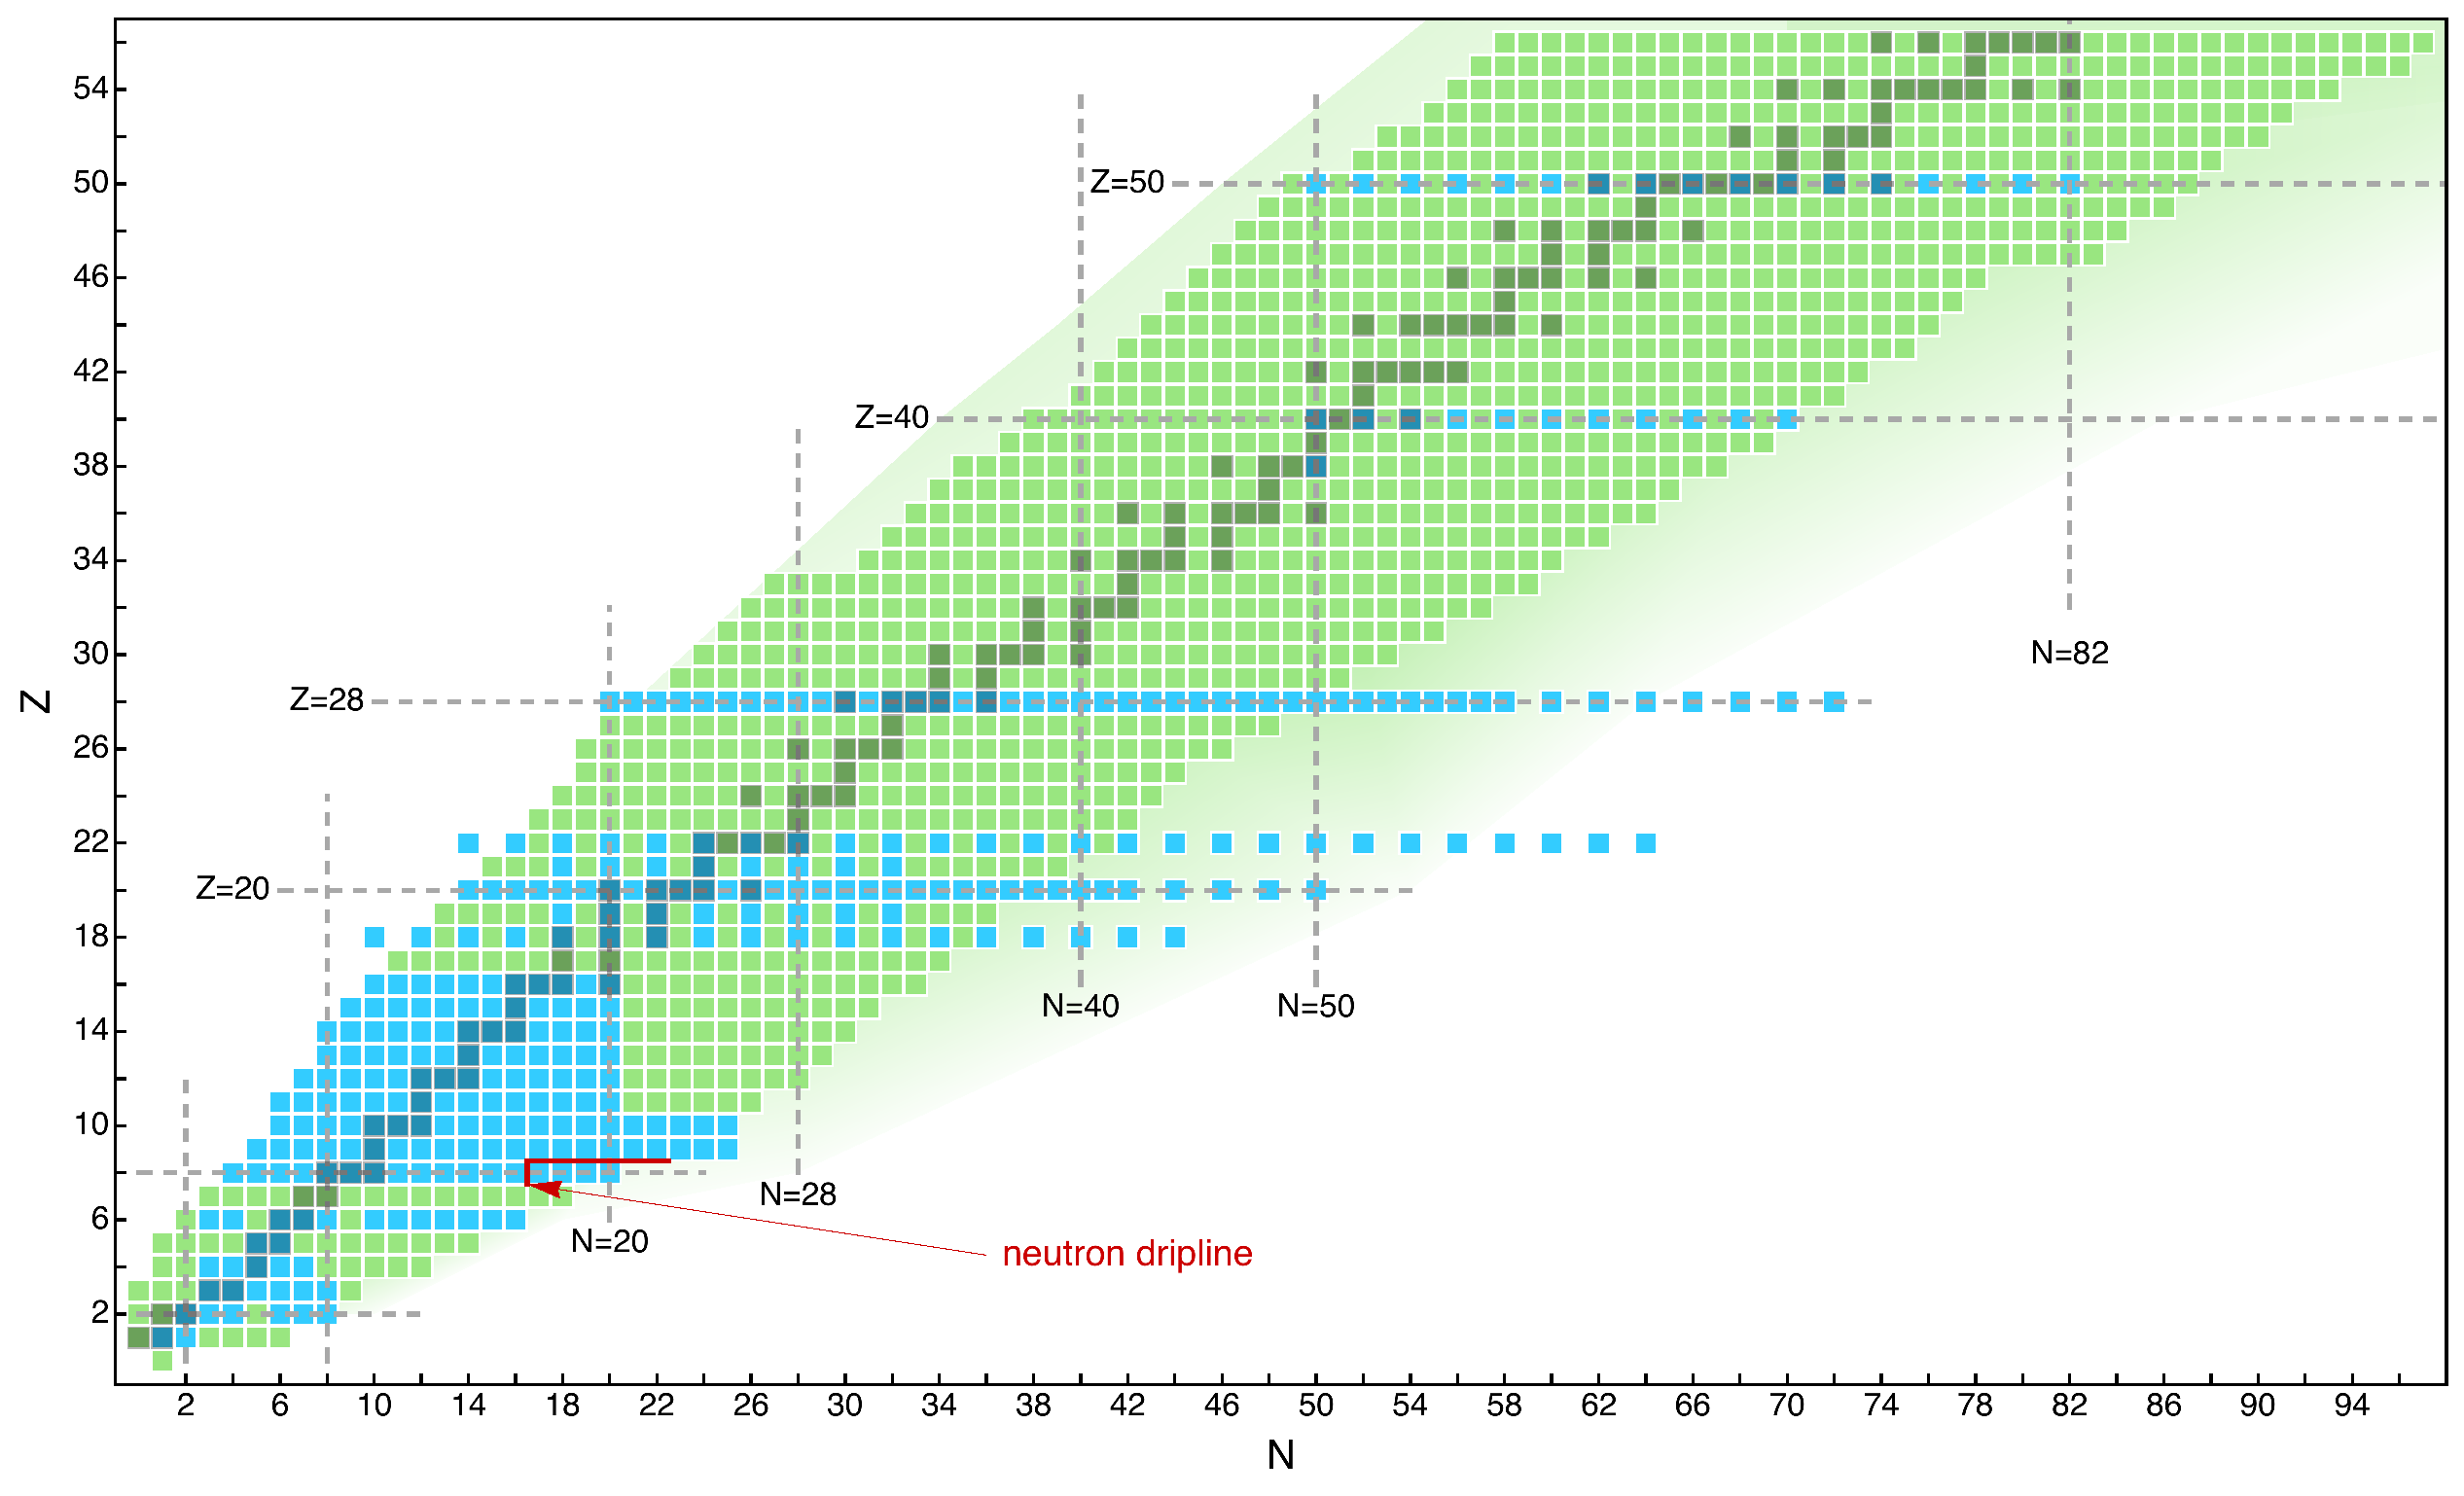
\includegraphics[width=.99\linewidth]{ab-initio_nuclear_chart_2015.eps}
%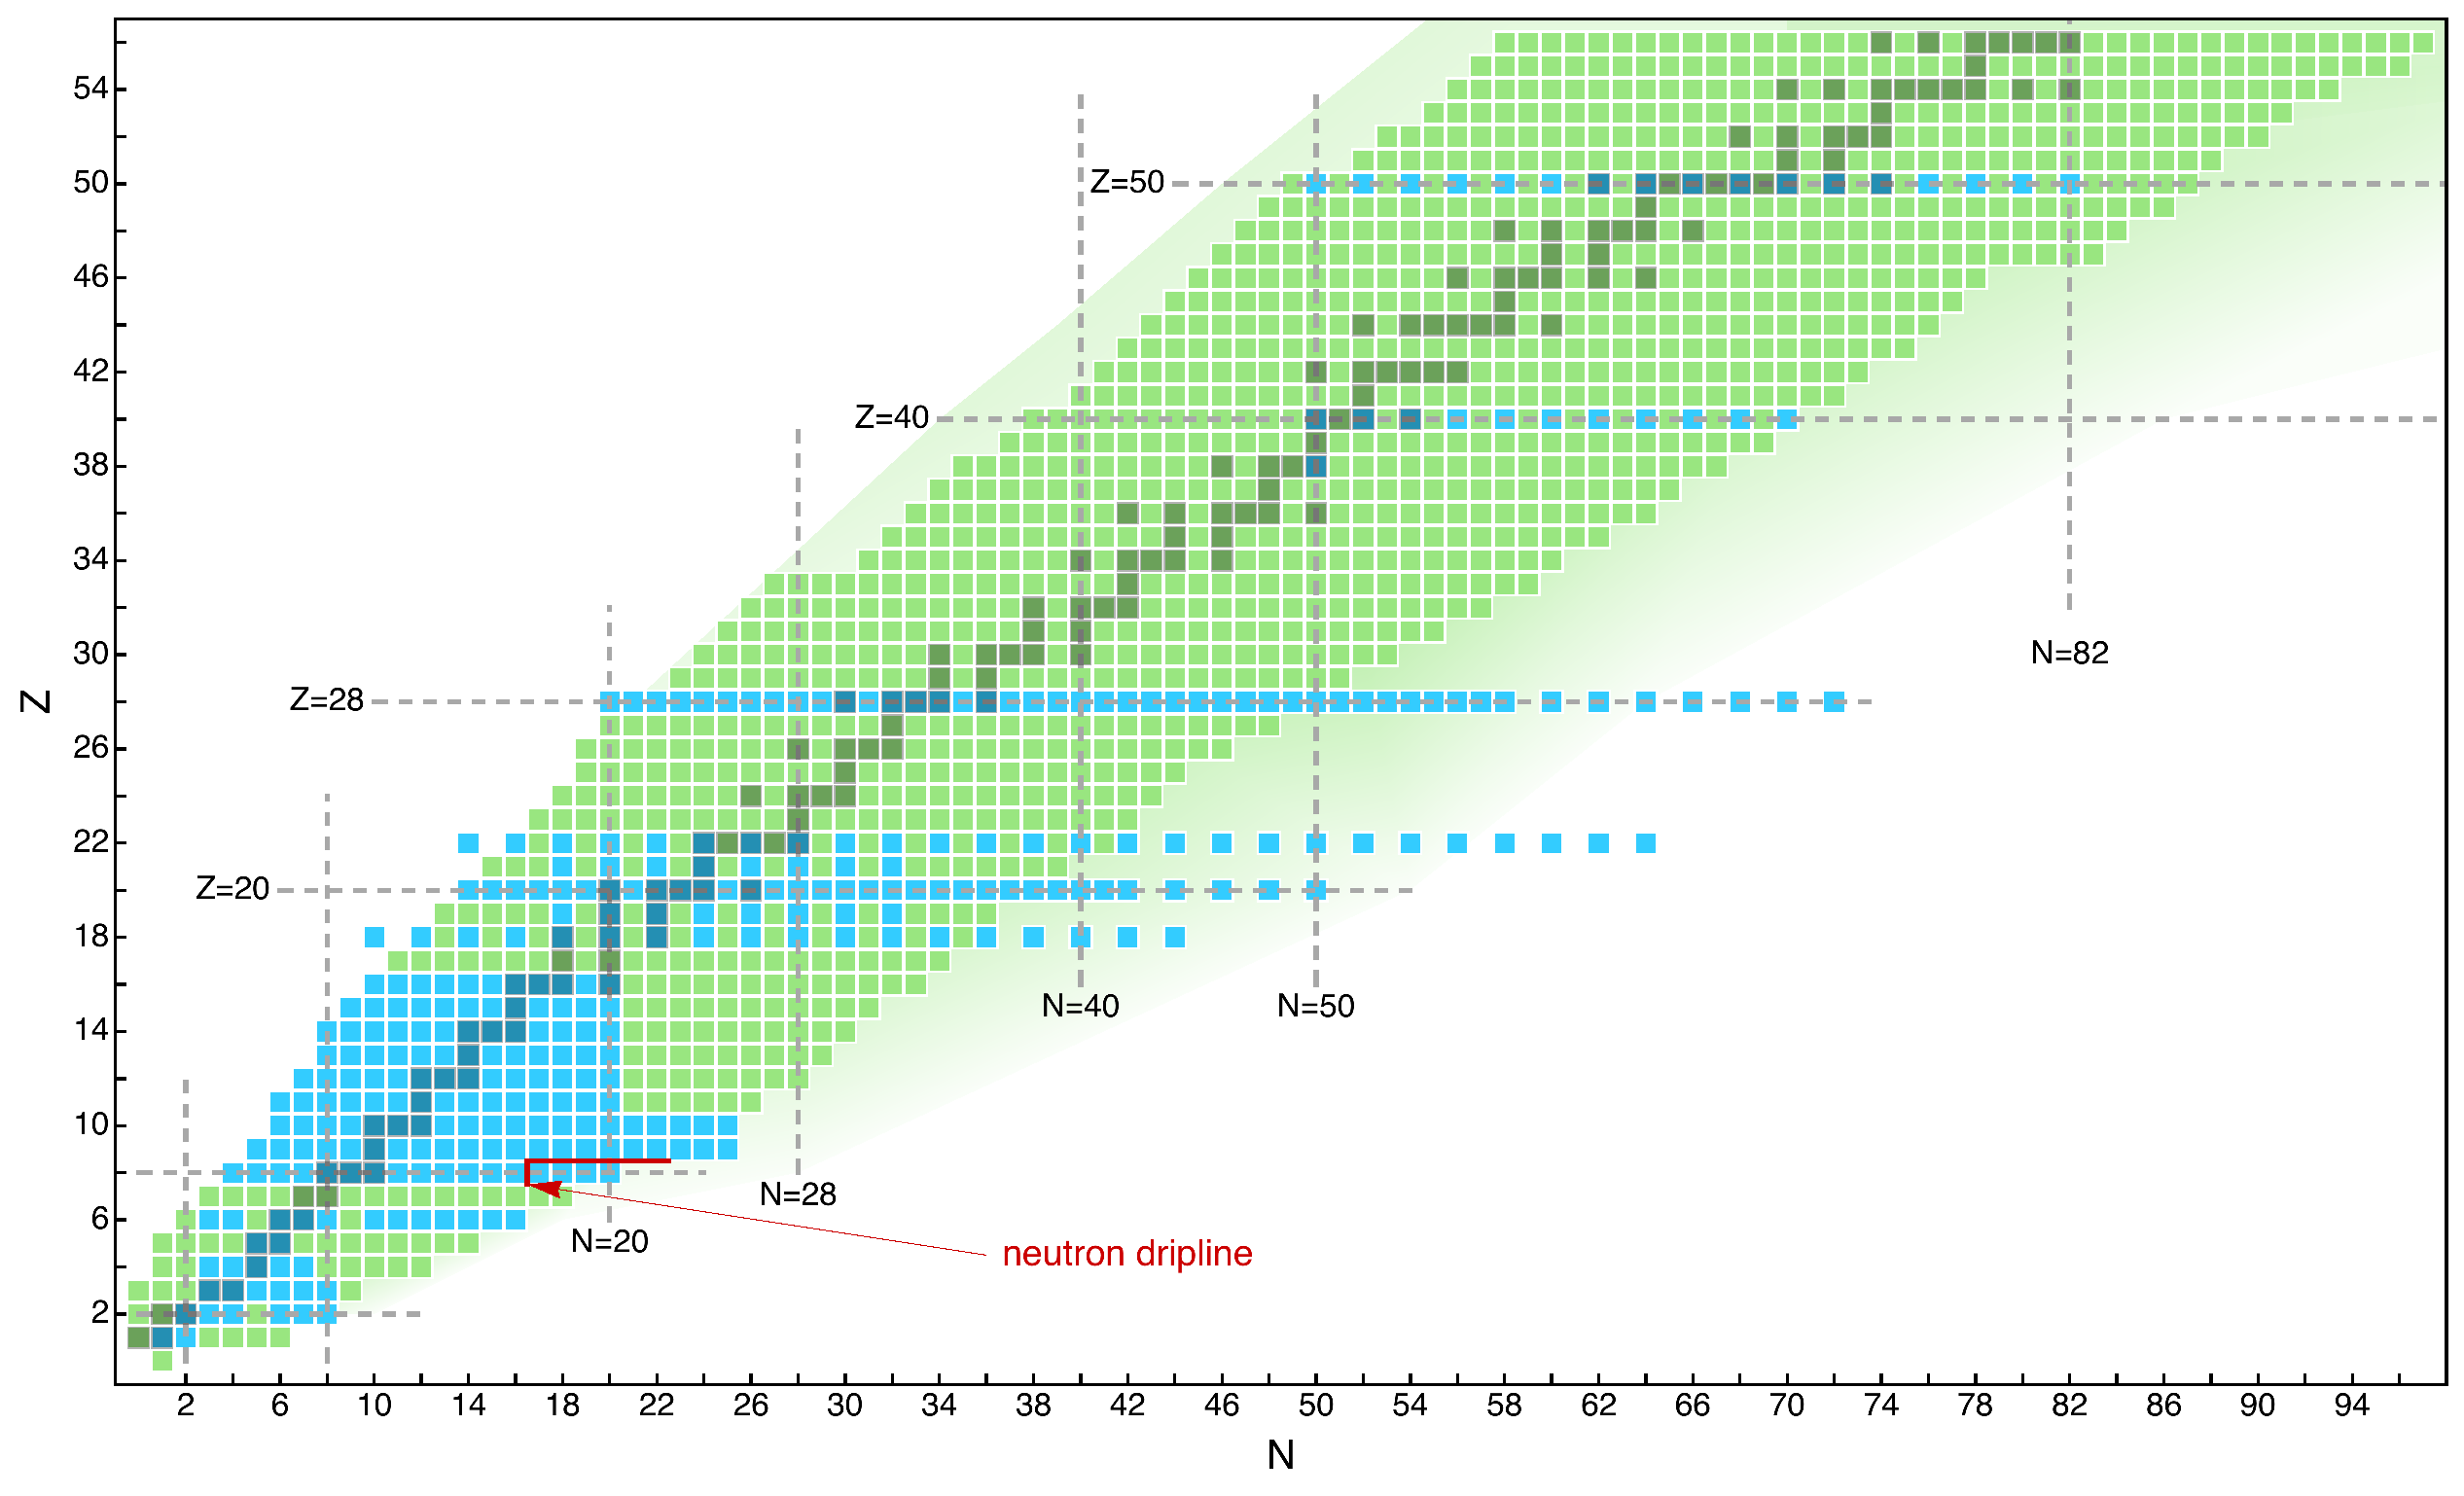
\includegraphics[height=3.0 in]{ab-initio_nuclear_chart_2015.eps}
   \caption{\label{fig:abinitio2015}}
\end{subfigure}
\caption{\label{fig:abinitio}The chart of nuclides and the reach of \emph{ab initio} calculations in (a) 2005 and (b) 2015. Nuclei for which \emph{ab initio} calculations exist are highlighted in blue. Note that the figure is for illustrative purposes only, and is based on the authors' non-exhaustive survey of the literature.}
\end{figure}

Both applicants have played significant roles in key developments that
have driven the progress shown in Fig.~\ref{fig:abinitio}. For
instance, on the interactions side Bogner has been closely involved
with the development of new RG technologies to evolve inter-nucleon
interactions and operators to softer
forms~\cite{Bogner:2001gq,Bogner:2006vp,Bogner:2006pc,Bogner:2010pq},
while Hjorth-Jensen has been actively involved with efforts to
generate improved chiral EFT interactions through the use of better
fitting protocols and advanced statistical
tools~\cite{Ekstrom:2013kea,Ekstrom:2014dxa,Ekstrom:2015rta}.  On the
many-body side, Bogner and collaborators were the first to introduce
the IMSRG framework to nuclear
physics~\cite{Bogner:2010pq,Tsukiyama:2011uq,Tsukiyama:2012fk}, and
have been centrally involved in many of the subsequent extensions and
applications of the
method~\cite{Hergert:2014vn,Bogner:2014tg,Morris:2015ve,Stroberg:2015ymf,Hergert:2015awm}. Likewise,
Hjorth-Jensen and collaborators initiated the revival of CC methods in
nuclear physics nearly 15 years ago~\cite{Dean:2002bx,Dean:2003vc} ,
and have been involved in most of the subsequent applications to
nuclei and nuclear
matter~\cite{Hagen:2012sh,Hagen:2013nca,Jansen:2011gb,Jensen:2011mv,Hagen:2016xjv}.



In the following, we present a research plan to develop a
comprehensive many-body framework based on CC and IMSRG methods that
seeks to fulfill the following general criteria: i) calculations must
make use of the best available chiral EFT two- and three-nucleon
interactions and come with controllable (i.e., quantifiable)
theoretical uncertainties, ii) approximations/truncations in the
many-body theory must be systematically improvable, iii) the formalism
must be able to account for the open-quantum-system aspects of loosely
bound and unbound nuclear states that couple to the continuum, iv) the
formalism should be capable of treating a range of systems from finite
nuclei (ground and excited states, open-shell and closed-shell,
well-bound and loosely-bound, etc.) to equation of state calculations
of infinite matter of relevance for studies of proto-neutron stars and neutron stars.


A complete theoretical picture which addresses this range of systems
requires a proper link between many different energy and length
scales\footnote{A simultaneous description of nuclei and neutrons
stars spans over 19 orders of magnitude, from several $10^{-15}$\,m
(nuclear radii) to approximately 10 kilometers (neutron star radii).}.
In nuclear physics, the optimal theoretical description is
``resolution dependent'', in that phenomena at each energy scale has
an appropriate (i.e., most convenient) effective theory and
corresponding set of degrees of freedom. One of the central challenges
for theory is to understand how connections between different
effective descriptions emerge at the boundaries.  This is an
interesting theoretical problem in and of itself, but it also carries
important practical implications. For example, phenomenological shell
model and density functional theory methods, both of which are
low-resolution descriptions, have been extremely successful in making
predictions and describing experiment \emph{in the vicinity} of the
data to which they were fit to, but tend to give uncontrolled
extrapolations away from this region.  One of the central aims of our
proposed research is to use controlled \emph{ab initio} calculations
(a high-resolution description) to constrain the form and values of
couplings in low-resolution shell model interactions and Skyrme-like
energy density functionals, with the goal of improving their
predictive power away from known data.


The methods in this proposal have the potential to
dramatically increase our understanding of a new frontier in nuclear
physics, namely the role of three-nucleon forces in the evolution
of nuclear structure and dense matter. Neutron-rich nuclei are particularly interesting
to study these effects~\cite{Otsuka:2009cs,Holt:2011fj,Holt:2014aya}, where
the modification of magic numbers, formation of neutron skins and
halos, and detailed tests of shell structure at the limit of
neutron-to-proton asymmetry can be probed via investigations of
masses, radii, and excited states~\cite{Wienholtz:2013bh,Hagen:2015ve,jansenprl2016}. Global theoretical
studies of long isotopic chains, such as the chains of calcium, nickel or
tin isotopes, make it possible to systematically test properties of
nuclear Hamiltonians and many-body methods.  A quantitative
comparison of various experimental data with quantified theoretical
uncertainties still remains a major challenge for nuclear science. To
address this shortcoming, a key component of our research will
be to seek a better understanding of the theoretical uncertainties
that arise from the interplay of truncation errors of the chiral EFT interactions, uncertainties in the
fitted parameters of the low-energy constants, truncated renormalization
group evolution to ``soften'' the input Hamiltonian, basis-set
truncation errors, and truncation errors in the particular level of
many-body approximation.

The development of {\em ab initio} many-body theories for nuclei is also
intimately linked with the determination and our understanding of the
equation of state (EoS) for nuclear matter.  The CC and IMSRG methods are both promising 
candidates to carry out controlled EoS
calculations starting from chiral NN and NNN interactions, due in
equal measure to their computational scalability and flexibility. Bulk nucleonic matter is
interesting for several reasons. The EoS of neutron matter, for
instance, determines properties of supernova
explosions~\cite{Sumiyoshi:2005ri,Murphy:2009dx} and neutron
stars~\cite{Hebeler:2014ema, Lattimer:2000kb, Lattimer:2000nx},
and it relates the latter to neutron radii in atomic
nuclei~\cite{Brown:2000pd, Horowitz:2000xj}. Likewise, the compressibility of
nuclear matter is probed in isoscalar giant monopole
excitations~\cite{Shlomo:1993zz}, and the symmetry energy of nuclear
matter is related to the difference between proton and neutron radii
in atomic nuclei~\cite{Abrahamyan:2012gp,Reinhard:2013fpa}. We also
note that the saturation point of nuclear matter determines bulk
properties of atomic nuclei, and therefore is an important constraint
for nuclear energy-density functionals and mass models~\cite{Kortelainen:2011ft,Bertsch:2004us}.  Finally, our calculations of in-medium
operators and interactions can be used to evaluate, with state-of-the-art Hamiltonians,
neutrino emissivities and spectra in dense objects like neutron stars and proto-neutron stars \cite{Balasi:2015dba,Lohs:2015qyn}.

Numerous components of our proposed
research mesh well with the research interests of other NSCL theory
faculty, which will lead to increased opportunities for
collaboration. Heiko Hergert, who is a former postdoc of Bogner and
who joined the faculty in 2015, has been (and will continue to be) a
frequent collaborator on IMSRG-related topics. Our research on
constructing \emph{ab initio} shell model Hamiltonians via CC,
IMSRG, and MBPT methods is complementary to the expertise of Alex Brown, who is
a leading shell model practitioner and developer of phenomenological
shell model interactions. Similarly, our proposed development of the
equation of state calculations is highly relevant to the research of
Pawel Danielewicz and Filomena Nunes on the nuclear symmetry energy
and transport theory for heavy-ion reactions, as well as new hire Luke
Roberts and his research on the role of neutrinos and core-collapse supernovae.




\subsection{Results from prior NSF support}

\subsubsection{Prior funding from 2011-present}
The PIs have received support as principal investigator or
co-investigator for the following grants since 2011:
\begin{itemize}
%\item NSF Grant No. PHY-0653312 
%\item DOE Grant No.  DE-FC02-07ER41457 
\item SciDAC UNEDF collaboration under DOE Grant No. DE-FC02-09ER41585 (B.~A. Brown and S.~K. Bogner, co-investigators from 2007-2012)
\item NSF Grant No. PHY-0758125 (S.~K. Bogner, PI from 9/1/2008 to 8/31/2011)
\item NSF Grant No. PHY-1068648 (S.~K. Bogner, PI from 7/1/2011 to 6/30/2014)
\item NSF Grant No. PHY-1404159 (S.~K. Bogner and M.~Hjorth-Jensen, Co-PIs from 9/1/2014 to 8/31/2017)
\item SciDAC NUCLEI collaboration under DOE Grant No. DE-SC0008511 (S.~K. Bogner, PI from 5/1/2012 to 4/30/2017)
\item Research Council of Norway contract No. ISP-Fysikk/216699 (M.~Hjorth-Jensen, from 6/1/2012 to 6/1/2016)
\end{itemize}



%There is a strong educational component in the PIs' research program,
%as well as within the MSU theory group as a whole. For instance, both PIs have played an
%active role in organizing and lecturing at the Nuclear TALENT summer schools 
%(Hjorth-Jensen serves on the TALENT advisory board). The graduate
%nuclear physics program at MSU is consistently ranked at the top of
%various rankings, and the theory group has enjoyed a very good track
%record in attracting the top graduate students at MSU, including
%members of underrepresented groups (e.g., the PI's first PhD student who graduated in 2011, Biruk
%Gebremariam).  In recent
%years, the number of theory students has steadily increased to the
%current value of approximately 2 students per PI. Students and
%postdoctoral researchers enjoy many professional development
%opportunities, such as the ability to interact with a wide range of
%nuclear physicists that visit the NSCL.


\subsubsection{Publications (2011-present)}
In the last five years, we have published 52 scientific articles in
peer-reviewed journals, these are listed under references below, see
\cite{Parzuchowski:2016njm,Stroberg:2016ung,Hergert:2015awm,Stroberg:2015ymf,Morris:2015ve,Caceres:2015fk,
  Morris:2014bwa, Konig:2014hma,Hergert:2014vn,Shirokov:2014kqa,Bogner:2014tg,Hergert:2012nb,Bogner:2012zm,Bogner:2011kp,Tsukiyama:2011uq,Tsukiyama:2012fk,Ormand:2016vup,Hagen:2016xjv,Tsunoda:2016fjh,Hagen:2015yea,Osnes:2015mte,Ekstrom:2015rta,Engeland:2014sya,Ekstrom:2014dxa,Vajta:2014wbx,Sanetullaev:2014uya,Balantekin:2014opa,Hagen:2013nca,Hagen:2013yba,Tsunoda:2013bla,Bader:2013npa,Baardsen:2013vwa,Ekstrom:2013kea,Lepailleur:2013bw,Liddick:2013vv,DiJulio:2013gq,Forssen:2012yn,DiJulio:2012fw,DiJulio:2012js,DiJulio:2012gk,Hagen:2012fb,Hagen:2012sh,Torres:2012zz,Torres:2011zz,Tsunoda:2011gh,Bergli:2010tz,Lohne:2010aw,Jensen:2011mv,Jansen:2011gb,Jensen:2010bd,
  Brown:2010ce,Signoracci:2010bz}.  In addition, we have recently
finalized a book on {\em Computational Nuclear Physics} to be published by
Springer under the Lecture Notes in Physics series. This book contains
two long chapters on Coupled Cluster theory and the IMSRG approach
applied to infinite nuclear matter and neutron star studies, co-authored with our graduate students
\cite{lnp}. In addition, two books on Computational Physics written by
Morten Hjorth-Jensen are to be published by the Institute of Physics
Publishing IoP, UK in 2017, see Refs.~\cite{book1mhj, book2mhj}.

\subsubsection{Workshops and programs organized (2011-present)}

Both PIs have been involved in the organization of several workshops
and schools during the last five years.  The Nuclear Talent
initiative, which Hjorth-Jensen initiated together with several
colleagues from Europe and the US, see \url{www.nucleartalent.org} for
more information, has now offered eleven courses in Nuclear Theory
since 2012, with approximately 40 applicants per course. Both PIs have
been active teachers and organizers of several Nuclear Talent
courses. This initiative has developed a broad nuclear physics curriculum, taught
through intensive three-week courses, that provides the
platform for a cutting-edge theory for understanding nuclei and
nuclear reactions.  This initiative has been well-received by the
nuclear physics community. In addition to the Nuclear Talent courses,
both PIs have been active in organizing other schools and
workshops/conferences.  During the last five years we have organized
11 schools, workshops and meetings. These are listed in the supplementary documentation.
%{\footnotesize
%\begin{enumerate}
%\item Hjorth-Jensen, Morten, {\em Computational Physics and Quantum Mechanical Systems}, one week course on Computational Physics at the University of Tunis El Manar, Tunis, Tunisia, May 16-20, 2016. In total 15 hours of lectures and 15 hours of computer lab and exercises.
%\item Hjorth-Jensen, Morten, co-organizer with Giuseppina Orlandini and Alejandro Kievsky of {\em Nuclear Talent course Few-body methods and nuclear reactions}, ECT*, Trento, Italy, July 20-August 7 2015
%\item Carlo Barbieri, Wim Dickhoff, Gaute Hagen, Morten Hjorth-Jensen, and Artur Polls, {\em Nuclear Talent course on Many-body methods for nuclear physics}, GANIL, Caen, France, July 5-25 2015. Main organizer and teacher as well with in total five hours of lectures.
%\item Bogner, Scott, Hjorth-Jensen, Morten, and Holt, Jason, {\em International Collaborations in Nuclear Theory:
%Theory for open-shell nuclei near the limits of stability}, organizers, Michigan State University, East Lansing, Michigan, May 11-29, 2015.
%\item Hjorth-Jensen, Morten, {\em Nuclear Talent School in Nuclear Astrophysics}, co-organizer with Richard Cyburt and Hendrik Schatz of the Nuclear Talent course on Nuclear Astrophysics, Michigan State University, May 26 - June 13, 2014.
%\item Bogner, Scott, Hjorth-Jensen, Morten,  Nicolas Schunck, Dario Vretenar and Peter Ring, {\em Nuclear Talent course on Density Functional theories}, European Center for Theoretical Nuclear Physics and Related Areas, Trento, Italy, July 13 -August 1 2014.
%\item Bogner Scott, {\em INT program on Computational and Theoretical Advances for Exotic Isotopes in the Medium Mass Region}, organizer with Carlo Barbieri, Thomas Duguet and Gaute Hagen, Institute of Nuclear Theory, University of Washington, Seattle, March 25-April 19, 2013.
%\item Hjorth-Jensen, Morten, {\em Nuclear Talent Course Introduction on High-performance computing and computational tools for nuclear physics}, ECT*, Trento, Italy, June 24 - July 13 2012. Main organizer and teacher together with Francesco Pederiva, Kevin Schmidt and Calvin Johnson.
%\item Bogner, Scott, {\em EMMI program The Extreme Matter Physics of Nuclei: From Universal Properties to Neutron-Rich Extremes}, 
%organizers with Thomas Aumann, Richard Furnstahl, and Achim Schwenk, 
%April 16 - May 11, 2012, GSI, Darmstadt, Germany.
%\item Hjorth-Jensen, Morten, organizer with David Dean, Thomas Papenprock and Gaute Hagen, {\em Third MSU-UT/ORNL-UiO winter school in nuclear physics}, Oak Ridge National Lab, Tennessee, January 2012
%\item Hjorth-Jensen, Morten, organizer with Alex Brown and teaching five lectures. {\em Second MSU-UT/ORNL-UiO winter school in nuclear physics}, East Lansing, Michigan, USA; 2011-01-03 - 2011-01-07

%\end{enumerate}
%}

\subsubsection{Guidance of students (2011-present)}

In the period of 2011-present, Bogner has supervised 7 graduate students at the NSCL. Of
these students, 2 have graduated with Ph.D.'s, 4
currently remain in the Ph.D. program under SB's supervision, and 1 has 
decided to leave with a Masters degree in Spring 2017.  The first
Ph.D. recipient (Biruk Gebremariam, 2011) is a software analyst for the
company SAS, while second Ph.D. recipient (Titus Morris, 2016) is presently
a postdoc at the University of Tennesse and Oak Ridge National Lab. Of the
4 current Ph.D. students, 3 are co-supervised with Morten Hjorth-Jensen,
see below.
 
Hjorth-Jensen started at MSU in January 2012, and spends half the year
(January-June) in the USA and the other half at the University of Oslo
in Norway. Norway follows the standard European setup for higher
education, where a Master of Science degree is compulsory in order to
enlist in a Ph.D. program.  The Master of Science degree consists of
one year of course work and one year of own research work, often
ending in a scientific article.  In the period 2011-2016, three
Ph.D. students and 22 M.S. students finalized their theses with
Hjorth-Jensen as supervisor. Of the three Ph.D. students, two are
presently post-doctoral fellows in Norway at the University of Oslo
while Gustav Jansen (PhD 2012) is now permanent staff at the
Computational Science Division of Oak Ridge National Laboratory. Of
the 22 M.S. students, 12 have continued with Ph.D.  studies in
Norway. Hjorth-Jensen presently supervises (either as primary or as
secondary supervisor) four Ph.D. students at MSU and eight
M.S. students at the University of Oslo. Three of the students at MSU
are co-supervised with Scott Bogner.


The applicants have a total of five graduate students at present. Nathan
Parzuchowski works with Bogner and will finish his Ph.D. by the end of
Spring 2017.  The primary topic of his thesis is the development of
new \emph{ab initio} methods to calculate excited-state properties
(spectra, transition densities, response functions, etc.)  in
medium-mass nuclei by merging Equation of Motion (EOM) methods with
the IMSRG.  He has been supported in part by Bogner's PHY-1068648,
PHY-1404159 and SciDAC NUCLEI grants since he joined the group in
Summer 2013.

The four remaining students, Justin Lietz, Sam Novario, Fei Yuan, and
John Bower are co-supervised by Hjorth-Jensen and Bogner.  All four
students have received partial support from NSF Grant No. PHY-1404159
and the SciDAC NUCLEI grant. Yuan joined the group in Fall 2013, and
is working on implementing the IMSRG in a complex Gamow basis to
properly treat continuum effects for loosely bound states. He is
projected to finish his Ph.D. by the end of Fall 2017. Lietz joined
the group in Fall 2013 and is projected to finish his Ph.D. in Spring
2018, with a focus on computational elements of coupled-cluster theory
and the IMSRG, with applications to infinite matter calculations to
constrain neutrino interactions in matter. Novario joined the group in
Summer 2014 after spending three years in the experimental nuclear
physics program.  He is expected to complete his Ph.D. by the end of
Summer 2017 on effective operators from coupled-cluster
theory. Bower joined the group in Summer 2015, and is going to leave
with Masters degree in Spring 2017.





\subsubsection{Results under prior NSF support: Intellectual Merit  }
In the present section, we give a brief summary of the \emph{intellectual merit} of the PIs accomplishments under prior NSF support from 2011-present.  We focus only on activities that are of primary importance to our proposed research. The \emph{broader impacts} of our prior NSF-supported research will be discussed below.
\begin{itemize}

\item{\bf In-medium SRG for Nuclei.} The Similarity
Renormalization Group (SRG) was developed in the early 1990's by
Wilson and Glazek~\cite{Glazek:1993il}, and by
Wegner~\cite{Wegner:1994dk}. In Ref.~\cite{Bogner:2006pc}, Bogner \emph{et al.} 
made the first applications of the SRG to low-energy nuclear
physics to soften two-nucleon interactions, which has since become a ubiquitous tool in \emph{ab initio} theory~\cite{Bogner:2010pq,Binder:2013zr,Hupin:2013uq,Roth:2011kx}.  Subsequently, Bogner and collaborators formulated an alternative version of the SRG  in which the evolution is performed ``in-medium'' (i.e., directly in the $A$-body system of interest) rather than in vacuum~\cite{Tsukiyama:2011uq, Tsukiyama:2012fk}.  In contrast to the free-space SRG, the
in-medium similarity renormalization group (IMSRG) approach enables one to approximately evolve $3,...,A$-body operators
using only two-body machinery based on normal-ordering
techniques. The IMSRG is a powerful \emph{ab initio} framework because it offers several paths to calculate ground and excited state properties for closed- and open-shell medium-mass nuclei, see for instance the two recent review articles~\cite{Hergert:2015awm,Hergert:2016etg}. 
%ranging from {\em ab initio} calculations of closed-shell nuclei and nuclear
%matter~\cite{tsukiyama2011,tsukiyama2012,hergert2012}, to the construction of
%effective valence shell-model Hamiltonians and multi-reference
%extensions of the IMSRG to treat open-shell
%systems~\cite{tsukiyama2012, Hergert:2013uja}.

%\begin{enumerate}

\item{\bf Ground-state IMSRG for closed-shell systems.} The IMSRG was originally developed to target the ground states of closed-shell systems~\cite{Tsukiyama:2011uq}. Over the past five years, calculations have been performed for all closed shell nuclei up thru $^{56}$Ni with initial three-nucleon forces~\cite{Hergert:2015awm, Hergert:2013mi}. Calculations have also been performed for non-nuclear systems like the electron gas, two-dimensional parabolic quantum dots, and diatomic molecules at equilibrium geometries~\cite{sarahthesis, TitusThesis}. In the simplest IMSRG(2) truncation, where the flow equations are truncated at the normal-ordered two-body level, ground-state energies track CCSD(T) calculations with approximate triples excitations more closely than the analogous CCSD results. This apparent higher-order accuracy was explained by analyzing the low-order MBPT content of the IMSRG(2) and CCSD approximations, where it was shown that the former undercounts a set of repulsive 4th-order terms by a factor of 1/2, which mimics the partial cancellation against attractive triples contributions~\cite{Evangelista, TitusThesis,Hergert:2015awm}.  
 
\item {\bf Magnus expansion formulation of the IMSRG.} In the traditional IMSRG formulation, one solves coupled ordinary differential equations (ODEs) for the evolved Hamiltonian matrix elements. To maintain unitary equivalence, it is necessary to use a high-order method to prevent the accumulation of ``time-step'' errors. High-order solvers can require the storage of 10-20 copies of the solution vector, resulting in a large memory overhead. The problem is exacerbated if one calculates additional observables, as the number of flow equations is roughly doubled in size for each. In Ref.~\cite{Morris:2015ve}, we showed how a naive first-order Euler method can be used to solve reformulated IMSRG equations without any degradation in accuracy. The new formulation uses the Magnus expansion to solve for the operator $\Omega$ that parameterizes the IMSRG unitary transformation $U = e^{\Omega}$, rather than solving flow equations for the Hamiltonian. The transformed Hamiltonian, and any additional observables of interest, can then obtained by the direct application of $U$. The resulting computational savings are substantial, and the calculation of additional observables carries almost no additional cost.  Additionally, the Magnus formulation provides a simple framework to construct computationally-feasible approximations to the IMSRG(3) truncation, which have been successfully implemented and tested for 2d quantum dots, the homogenous electron gas, and diatomic molecules at equilibrium and stretched geometries~\cite{TitusThesis}.   

 \item {\bf \emph{Ab initio} construction of shell model
 interactions.} For open-shell nuclei, one promising approach is to
 use the IMSRG to construct a valence-space Hamiltonian that is diagonalized using shell model
 machinery.  In Ref.~\cite{Bogner:2014tg}, the first IMSRG calculations of valence-space Hamiltonians 
 based on chiral two- and three-nucleon interactions 
 were presented. When applied to the neutron-rich oxygen isotopes,
 natural-parity spectra are in excellent
 agreement with experiment. However, ground-state energies show systematic overbinding as more
 neutrons are added due to the neglect of
 three-nucleon interactions among valence nucleons.  In two
 subsequent works~\cite{Stroberg:2015ymf,Stroberg:2016ung}, this was
 remedied using improved normal ordering procedures. The improved formulations correct the ground-state
 systematics, bringing the valence space calculations into excellent
 agreement with the large-space methods for a wide range of isotope
 chains from Carbon thru Nickel. Additionally, ``emergent phenomena''
 such as Yrast rotational bands in deformed nuclei such as $^{24}$Mg
 and $^{20}$Ne are accurately captured in our \emph{ab initio} shell model
 approach. The inclusion of initial three-nucleon forces improves
 spectra for a wide range of isotope chains, clearly demonstrating
 their importance in \emph{ab initio} studies of nuclear structure.
 
 \item {\bf Multi-reference formulation of the IMSRG.} The
 multi-reference formulation of the IMSRG (MR-IMSRG) is an appealing alternative to target open-shell
 systems~\cite{Hergert:2013ij} that bypasses the
 large-scale matrix diagonalizations required for
 midshell nuclei and/or extended valence spaces. In the MR-IMSRG, the
 ground states of even-even nuclei are targeted directly by using a
 number-projected Hartree Fock Bogoliobuv (HFB) reference state. In
 Ref.~\cite{Hergert:2014vn}, the method was used to calculate
 even-even ground states for Nickel and Calcium chains starting from
 chiral two- and three-nucleon interactions. At sub-shell closures,
 the MR-IMSRG results are in excellent agreement with CC calculations,
 and clearly show the importance of initial three-nucleon interactions
 to obtain a correct reproduction of experimental energy trends.
 
 \item {\bf EOM-IMSRG for excited states.}  In
 Ref.~\cite{Parzuchowski:2016njm}, we presented a new approach to 
 calculate excited states in medium-mass nuclei by merging 
 equations-of-motion (EOM) techniques~\cite{Rowe:1968eq} with the IMSRG. 
 Proof-of-principle calculations were performed for parabolic
 quantum dots in two-dimensions and the closed shell nuclei $^{16}$O
 and $^{22}$O.  The calculated spectra are in reasonable agreement with
 analogous EOM-coupled-cluster (EOM-CC) calculations, which paves the
 way for more interesting applications such as calculations of electromagnetic strength functions and transitions,
 extensions to nuclei within 1-2 nucleons of a closed shell, and merging the EOM with the MR-IMSRG to 
 access open-shell nuclei.
%\end{enumerate}

\item {\bf \emph{Ab initio} studies of infinite nuclear matter.}
  Studies of dense baryonic matter are of central importance to our
  basic understanding of the stability of nuclear matter, spanning
  from matter at high densities and temperatures to matter found
  within dense objects like neutron stars. In four recent publications we have studied the equation
  of state for dense nuclear matter using CC theory in a
  cartesian basis. We have performed CC calculations at the CCD and CCD(T) levels (doubles and triples excitations, respectively) with and
  without chiral three-body forces
  \cite{Baardsen:2013vwa,Hagen:2013yba}.  These calculations agree
  well with results from quantum Monte Carlo computations. We found that
  neutron matter with interactions from chiral EFT is almost perturbative,
  while symmetric nuclear matter requires nonperturbative
  approaches, with correlations beyond the standard particle-particle
  ladder approximation yielding non-negligible contributions. The
  saturation point of symmetric nuclear matter is sensitive to the
  employed NNN forces and the employed regularization scheme.

  In two recent book chapters to be published in the series Lecture
  Notes in Physics by Springer \cite{lnp}, see also the discussion
  below on broader impacts, we have together with our graduate students
  and other colleagues, detailed the development of a
  computational many-body scheme for infinite nuclear matter using
  both CC theory and IMSRG. The codes and formalism exposed in this
  texts shows how to evaluate correlations at the level of $2p-2h$
  excitations for CC theory (CCD, doubles only) and IMSRG (IMSRG(2)). These codes can easily be
  extended to include more complicated correlations as well as
  realistic chiral interactions. The work here lays the foundation for
  our future plans described in the project description section.


\item {\bf \emph{Ab initio} Properties of nuclei with optimized
    nuclear Hamiltonians.}  Together with external collaborators, we have developed predictive
  {\em ab initio} nuclear hamiltonians for light and medium-mass
  nuclei with two-nucleon and three-nucleon forces from chiral
  effective field theory.  The parameters of these potentials have
  been optimized simultaneously to low-energy nucleon-nucleon
  scattering data, as well as binding energies and radii of
  few-nucleon systems and selected isotopes of carbon and
  oxygen. When used in many-body calculations, the optimized Hamiltonians yield results in close agreement with
  experiment also for nuclei not included in the fit
  \cite{Ekstrom:2015rta,Ekstrom:2013kea,Ekstrom:2014dxa}. Our recent
  applications to studies of the neutron and weak-charge distributions
  of $^{48}$Ca \cite{Hagen:2015yea} yield an excellent agreement with data. These results indicate that the neutron skin
  (difference between the radii of the neutron and proton
  distributions) is significantly smaller than previously
  thought. These calculations can in turn provide a constraint on the
  size of a neutron star.  Our progress in CC theory is
  summarized in two recent reviews~\cite{Hagen:2014ve,Hagen:2016xjv}.



\item {\bf Many-body perturbation theory and shell model
    interactions.}  In close collaboration with colleagues in Japan,
  we have extended our degenerate MBPT formalism (appropriate for one
  major shell only) to non-degenerate MBPT, allowing for studies of
  nuclei with degrees of freedom arising from more than one major
  shell.  In Ref.~\cite{Tsunoda:2016fjh} we applied the newly developed
  formalism to studies of exotic neutron-rich medium-mass nuclei.  The
  effective shell-model interactions derived using non-degenerate MBPT
  \cite {Tsunoda:2016fjh,Tsunoda:2013bla} were used to study
  energies and transition probabilities of neutron-rich Ne, Mg and Si
  isotopes. These are nuclei in the so-called {\em island of
    inversion} mass region. Previous shell-model studies of these systems
  have used phenomenologically tuned interactions. In
  Ref.~\cite{Tsunoda:2016fjh} we showed that a proper derivation of
  multi-shell effective interactions and the inclusion of three-body
  forces result in a better description of experiment, without the
  need of fine-tuning selected matrix elements.


\item {\bf CC and IMSRG calculations of quantum dots.} We have also
  performed extensive studies of quantum dots using IMSRG and CC
  theory, together with our MBPT and FCI codes as well as our
  diffusion Monte Carlo (DMC) codes. The DMC results serve as
  benchmark for the other methods. We find an excellent agreement
  between CC theory and IMSRG at the CCSD and IMSRG(2) levels of approximation
  for closed-shell systems with up to $N=56$ electrons. The CC
  and IMSRG results agree also well with the quasi-exact DMC results.
  Using the EOM-IMSRG discussed above and the analogous EOM-CCSD
  approach we have also evaluated the addition and removal energies
  for the same closed-shell systems. These results are
  obtained as a collaborative effort between three of our graduate
  students (Novario, Parzuchowski and Yuan) and will be published early 2017.
\end{itemize}

\subsubsection{Results under prior NSF support: Broader impacts }

One of our aims during the previous grant period was to develop an
open source library that can be used by other nuclear theorists and/or
serve students and post-doctoral fellows as a resource for learning
about advanced methods like CC theory and the IMSRG.  In our recent
Lecture Notes in Physics book (to be published in early 2017)
entitled {\em An advanced course in computational nuclear physics;
Bridging the scales from quarks to neutron stars} and edited by MHJ,
Van Kolck and Lombardo, we have together with our graduate students
and other colleagues, written two long chapters on the application of
the above many-methods to neutron matter. These chapters contain
links to our codes, which are fully open source and contain
benchmark calculations to ensure reproducibility of results. The text focuses on how to
develop large-scale many-body codes, with infinite neutron and nuclear
matter as examples, starting with a serial code and ending up with final product that can be tailored to present high-performance computing
facilities. The codes are accesible from the GitHub
link \url{https://github.com/ManyBodyPhysics/LectureNotesPhysics/tree/master/doc/src}. Many elements of the text have also entered
different courses we teach, in particular the various Nuclear Talent
courses that we have developed for the larger nuclear physics community. The text and associated codes can freely be used by our
colleagues in advanced nuclear physics courses elsewhere. 




%%%   Important note: think of a good write of the educational plan, that
%%is our plans fro training. Now it says nothing
\subsection{Proposed Research}


In this section, we describe the detailed components of our proposed research that was 
outlined in the Overview section. In the following project descriptions, Bogner will lead the 
IMSRG-related developments, while Hjorth-Jensen will lead the coupled-cluster theory developments.



\subsubsection{{\em Ab initio} calculations of Finite Nuclei}\label{subsec:finitenuclei}

The projects in this subsection concern the development of {\em ab
  initio} methods to calculate ground- and excited-state properties of
medium mass nuclei. The methods we will focus on are the IMSRG and CC theory. Since we
have already developed a large MBPT and large-scale FCI framework \cite{Hjorth-Jensen:1995ys,mhj2004,Tsunoda:2013bla,Tsunoda:2016fjh}, these methods will serve as
additional many-body methods used to compare our calculations with.
Emphasis will be placed on developing reliable and efficient {\em ab initio}
calculations of ground- and excited-state properties for both closed-
and open-shell nuclei, with the proper inclusion of two- and
three-nucleon forces and continuum degrees of freedom.  Additionally,
these developments will be used to inform and improve existing
phenomenological approaches, for instance by generating improved
starting points for the optimization of phenomenological shell model
Hamiltonians and energy density functionals, or by providing
qualitative insights as to the different types of couplings one
expects.



\begin{enumerate}
 
 \item {\bf Inclusion of NNN forces and three-body correlations.} 
 In the same way that NN interactions imply that, at a minimum, doubles excitations ($2p2h$,
  disconnected $4p4h$, etc.) must be included for an accurate
  description of many-body correlations, the presence of NNN forces
  demands an explicit treatment of triples excitations. We propose to 
  develop computationally feasible schemes for including explicit
  three-body correlations in CC and IMSRG calculations when NNN forces are present.  In CC theory, this corresponds to including
  non-iterative triples (e.g., CCSD(T)) and analogous approximations to full triples, while for the IMSRG, this entails performing approximate IMSRG(3)
  calculations using the Magnus expansion formulation developed in Refs.~\cite{TitusThesis, Morris:2015ve}. 
s
\item{\bf Merging EOM methods with the single-reference IMSRG.}
In Ref.~\cite{Parzuchowski:2016njm}, we presented a new approach to 
 calculate excited states in medium-mass closed-shell nuclei by merging 
 equations-of-motion (EOM) techniques~\cite{Rowe:1968eq} with the IMSRG.  We propose to extend this method to calculate ground- and excited-state properties of nuclei within 1-2 nucleons of a closed shell by extending the EOM ladder operators to include particle-number non-conserving terms. We will also use Lanczos' method and appropriately evolved operators to calculate nuclear response functions and transition densities. In principle, the same Lanczos techniques can be used to construct microscopic optical potentials when applied to the closed-shell $\pm 1$ nuclei, thereby linking \emph{ab initio} structure to reactions.
 
\item {\bf Merging EOM methods with the multi-reference IMSRG.}  The
  valence-space IMSRG~\cite{Tsukiyama:2012fk,Bogner:2014tg,
    Stroberg:2015ymf,Stroberg:2016ung} has the virtue of providing a
  unified treatment of ground- and excited-state properties couched in the familiar language of the shell model, but it also suffers the same ``curse
  of dimensionality'' associated with the large-scale matrix
  diagonalizations required for midshell nuclei and/or
  extended valence spaces.  One alternative is to directly target excited states by combining the
  IMSRG with equations-of-motion (EOM) techniques~\cite{Rowe:1968eq},
  similar to what is done in CC
  theory~\cite{Ekstrom:2014iya,Jansen:2012ey}. Successful
  ``proof-of-principle'' calculations have been performed in
  Ref.~\cite{Parzuchowski:2016njm}, where EOM methods were combined
  with the single-reference IMSRG to calculate excited states in
  closed-shell systems. While the EOM-IMSRG potentially offers some
  technical simplifications due to the Hermiticity of the transformed
  Hamiltonian (e.g., no need to solve a separate left-eigenvalue
  problem when calculating properties other than energy), the
  practical limitations of the single-reference formulation should be
  comparable to the analogous EOM-CC calculations, limiting the method
  to nuclei within 1 or 2 nucleons of a closed shell. To remove these
  limitations, we propose to merge EOM techniques with the
  multi-reference IMSRG (MR-IMSRG) formulation recently developed for
  ground-state calculations of open-shell even-even
  nuclei~\cite{Hergert:2013ij,Hergert:2014vn}. In principle,
  spectroscopy for the target nucleus and its even-odd, odd-even, and
  odd-odd neighbors could then be accessed using suitably generalized
  EOM excitation operators. This work will be done in close collaboration with
  NSCL colleague Heiko Hergert.
  
\item {\bf Continuum effect via the Gamow basis.}  As one nears the
  limits of stability, \emph{ab initio} calculations in a localized,
  $L^2$ single-particle basis fail to account for important couplings
  to resonances and the non-resonant continuum. In recent years, we
  have had success in working with the so-called Gamow basis in MBPT
  and coupled cluster calculations for nuclei near shell closures, see
  Ref.~\cite{Hagen:2006pq,Tsukiyama:2009hy,Hagen:2012oq} and
  references therein. To date, none of the IMSRG implementations have
  incorporated this important physics. Therefore, a major component of
  this proposal will be to implement the Gamow basis in the EOM-IMSRG,
  valence-shell decoupling IMSRG, and MR-IMSRG formulations, with
  particular emphasis placed on the latter two since they span the
  more challenging regime of unstable, open-shell nuclei. 
%  Our multi-shell MBPT formalism wil be extended in order to 
%include continuum effects as well as three-body forces, providing thereby three different many-body approaches to the inclusion of continuum effects.
  
\item {\bf Shell model interactions in extended valence spaces.} 
As one nears the limits of stability, traditional shell model calculations in a
single major shell are often insufficient. Moreover, for loosely-bound
systems it is necessary to utilize a single-particle basis which
accounts for resonances and the non-resonant continuum. Therefore, it
is a high priority to develop a framework to derive
multi-shell effective interactions with the proper inclusion of
continuum degrees of freedom using both CC and IMSRG methods. We note that we have recently tested multi-shell
effective interactions derived in MBPT for selected nuclei, see
Ref.~\cite{Tsunoda:2013bla,Tsunoda:2016fjh}. We propose to extend the CC effective interaction (CCEI)~\cite{Jansen:2014qf,Jansen:2015ngw} and the valence-decoupled
IMSRG methods~\cite{Bogner:2014tg,Stroberg:2015ymf,Stroberg:2016ung}, both of which have been quite successful in calculations within a single major shell and neglecting continuum effects, to the more
challenging case of multiple major shells within the Gamow basis.  Together with the previous item and with our
multi-shell effective interactions from MBPT, we have the possibility to test three different many-body approaches, with and without three-body forces and continuum effects.


\item{\bf Microscopically-improved phenomenological shell model
    interactions.}  In the phenomenological approach to shell model
  interactions, the valence single-particle energies (SPEs) and
  two-body matrix elements (TBMEs) are optimized directly to data. In
  practice, this is done by starting with some microscopic
  calculation, and then iteratively adjusting the relevant linear
  combinations of SPEs and TBMEs that are probed by the data, leaving
  the remaining terms fixed at the values given by the microscopic
  calculation~\cite{Brown:1988vm,Brown:2001rg,Caurier:2005qf}. In all
  applications to date, the microscopic starting point is taken from a
  low-order MBPT calculation without initial NNN forces. We propose to
  use our multi-shell MBPT, CCEI and IMSRG shell model interactions, which start from
  state-of-the-art chiral NN and NNN interactions, as an improved starting point for the
  optimization of phenomenological interactions in collaboration with NSCL colleague Alex Brown. We will also use
  qualitative and semi-analytic insights gleaned from the CCEI and
  IMSRG calculations to suggest alternative ans\"atze for the
  phenomenological interactions. For instance, in traditional
  phenomenology, the TBMEs are essentially fixed across the entire
  shell, with the exception of an empirical $A$-dependent scaling that
  mocks up the changing size of the
  core~\cite{Brown:1988vm,Brown:2001rg}. In contrast, the IMSRG
  valence interactions seem to suggest a much more complicated
  $A$-dependence~\cite{Stroberg:2015ymf,Stroberg:2016ung}.  We will
  also explore how the initial Hamiltonian is renormalized under the
  IMSRG to gain some insight into the general operator structures that
  result, which can then be used to motivate a ``bottom-up''
  description of the shell model as an effective field theory around
  the Fermi surface, in analogy with the modern RG view of
  Landau-Migdal theory~\cite{ShankarRG,MigdalBook}.
    
\end{enumerate}



\subsubsection{{\em Ab initio} calculations of infinite matter}\label{subsec:infinitematter}

Starting from optimized chiral EFT Hamiltonians we will perform extensive
studies of the equation of state of nucleonic matter, extracting
constraints on the energy per particle in symmetric matter and
$\beta$-stable matter, and obtaining reliable estimates for the
symmetry energy.  Our research aims at providing a consistent approach to several crucial quantities of relevance
for dense matter studies, spanning from the equations of state and the symmetry energy 
to various response functions and the estimation of  neutrino rates, spectra and opacities. These are all
quantities which play prominent roles in  our understanding of the evolution of neutron stars and proto-neutron stars.
The role of three-body forces on these quantities will be explored as well using realistic chiral Hamiltonians.

\begin{enumerate}
\item{\bf EoS and symmetry energy calculations.} We will develop IMSRG and CC calculations of
  the EoS and the symmetry energy of infinite matter starting from
  realistic NN and NNN interactions with approximate and full triples excitations. In our contributions to a recent
  volume of Lecture Notes in Physics (to be published in early
  2017), entitled {\em An advanced course in computational nuclear
   physics; Bridging the scales from quarks to neutron stars}
  \cite{lnp} (see also Refs.~\cite{Baardsen:2013vwa,Hagen:2013yba}), we have
  developed IMSRG and CC infinite matter codes at the IMSRG(2) and CCD levels of approximation. Building on this foundation,
  we will develop approximate IMSRG(3) and CCDT codes that are capable of treating realistic chiral NN and NNN interactions. These calculations will provide reliable   benchmarks for the EoS of general asymmetric nuclear matter and
$\beta$-stable nuclear matter. We have already implemented approximate 
  triples correlations in studies of the homogeneous electron gas for the coupled-cluster
  \cite{audunthesis} and IMSRG~\cite{TitusThesis} methods. Due to large memory requirements, our codes will need to be rewritten in order to run efficiently on existing and
  future high-performance facilities.  Finally, in addition to providing valuable information about the symmetry
  energy and its dependence on various components
  of the underlying NN and NNN interactions, these
  calculations will allow us to extract the so-called Landau fermi
  liquid parameters, which are useful to parameterize the collision
  integral term in transport theory.  This will naturally complement
  the reaction theory program of our colleagues Danielewicz and Nunes at the
  NSCL at Michigan State University.

% Should ask Luke to take a look at this? 

\item{\bf Effective operators and Neutrinos properties.} The CC and
  IMSRG methods will also allow us to extract one- and two-body
  effective operators for asymmetric infinite matter and to study
  their dependence on the various components of chiral NN and NNN
  interactions.  As an example, we will develop formalism and codes
  for computing effective baryon masses in dense matter as well as
  effective medium-dependent interactions and operators. These
  ingredients form the basis for the evaluation of various processes
  for neutrino emissions in dense matter. In neutron stars, neutrinos
  exhibit a mean free path which is larger than the typical radius
  $R\sim 10$ km of a neutron star. Neutron stars are thus expected to
  cool via various neutrino emission mechanisms such as the direct and
  modified Urca processes, and neutrino-pair bremsstrahlung. To
  properly account for the medium dependence of these processes, one
  needs controlled calculations of quantities such as nucleon
  effective masses, effective operators and interactions, and
  spin-isospin response functions. These elements all enter the
  determination of the rates that characterize the different neutrino
  production mechanisms. Normally, these have been approximated
  through various mean-field approaches or simplified phenomenological
  interactions. Changes in such rates due to uncertainties in
  different many-body methods can significantly alter the
  neutrino cooling timescale of proto-neutron stars and impact
  predictions of nucleosynthesis in the innermost regions of core
  collapse supernovae.  For instance, a proper knowledge of the
  spin-isospin response from {\em ab initio} methods, even in a
  limited range of temperature-density space, would provide valuable
  constraints on the phenomenological models that are in current
  use. The aim of this part of the project is thus to compute neutrino
  emissivities and spectra in dense matter using medium dependent
  quantities like effective masses, effective one-body operators and
  two-body interactions, and spin-isospin response functions extracted from IMSRG and CC calculations with
  and without NN and NNN forces. The hope is then to be able to
  provide better constrained predictions for neutrino spectra in dense
  matter.

  
\item{\bf Finite size corrections and many-body approximation errors.}
 In this subproject, we will treat the results from our large-scale simulations as ``synthetic data''  that depend on the number of basis functions used and the truncations
we make at the level of many-body excitations. By analyzing trends and correlations within the data, we will extract empirical guidelines and ``rules of thumb'' to estimate the theoretical uncertainties of common many-body approximations. 

  Since we simulate infinite matter in a finite periodic box and truncated plane-wave basis for both the
  IMSRG and CC methods, an important aspect will be to study and
  quantify finite-size and basis-truncation errors. For the former, we propose to study the use of
  so-called twisted periodic boundary conditions, which have been used
  with much success in condensed matter calculations to minimize
  finite size effects~\cite{Shepherd:2012,Hagen:2013yba,Drummond:2008}.  In
  depth studies of a proper treatment of finite size effects will be
  included in both our IMSRG and CC codes. Our numerical results for a wide range of basis sets will allow us to extract
  a better understanding of the basis-set truncation errors. An analysis along the lines performed
  by Shepherd in \cite{shepherd2016} will be done using our numerical data.
   
  We will also investigate truncation errors arising from different
  levels of many-body approximation. Unlike the studies of basis-set
  truncation errors, it is difficult to obtain an analytic or
  semi-analytic understanding of many-body approximation errors for
  nuclear many-body systems. Therefore, we will proceed in an
  empirical fashion by using benchmark results provided from auxiliary field diffusion Monte
  Carlo calculations~\cite{Roggero:2013ora,Roggero:2014lga,pederiva2016} to generate quasi-exact 
  results for a range of nuclear densities.  Using the
  Monte Carlo results as the exact benchmark, we will study how the
  truncation errors of the IMSRG, CC, and MBPT in different levels of approximation
  correlate with various quantities that one expects to affect convergence, such as the UV cutoff in the nuclear
  Hamiltonian, the D-state probability in the deuteron, the wound
  parameter calculated in leading-order Brueckner Hartree-Fock theory,
  etc. It is hoped that in this manner, we can at least gain ``rule of
  thumb'' estimates of how accurate we expect a given level of CC or
  IMSRG calculation to be given some simple quantities that
  characterize the input interactions and the reference state upon
  which correlations are to be built.   The calculations will be performed with and without three-body forces as well as with simplified Hamiltonians like those provided from pionless effective field theory \cite{pederiva2016}. The latter references, based on 
auxiliary field diffusion Monte Carlo calculations provide near exact benchmarks to neutron matter and symmetric nuclear matter calculations. 
 \end{enumerate}


\subsubsection{Applications to other systems}\label{subsec:othersystems}
To further validate our many-body machinery, we will also carry out
ground- and excited-state calculations using CC, IMSRG and MBPT
for the following well-studied systems that can serve as interesting
benchmarks for our methods:
\begin{enumerate}
\item{\bf Homogenous electron gas (HEG) in two and three dimensions.}
  The HEG has been studied extensively in the literature, see for
  example the recent full configuration interaction theory quantum Monte Carlo (FCIQMC) calculations of Alavi {\em et al}
  \cite{booth2009,booth2013}. We have recently started to study the
  two-dimensional HEG using CC theory and IMSRG,
  with very promising results~\cite{Baardsen:2013vwa,audunthesis}. These systems can
  serve as a testbed for the development of reliable infinite nuclear
  matter calculations, as much of the formalism is similar except that
  the nuclear forces have a finite range compared with the Coulomb
  interaction. Since Coulomb interactions are simpler, studies of the
  HEG will allow us to gain important insights about many-body
  correlations and various approximations like CC theory with and
  without triples correlations, IMSRG(2) and IMSRG(3) etc. In our
  IMSRG, CC and MBPT calculations to date, periodic boundary
  conditions have been used without including finite-size
  corrections~\cite{Baardsen:2013vwa, audunthesis}. Here again we plan to perform calculations with full triples
 and perform similar benchmark calculations as done for our nuclear matter calculations. 
  In order to compare the results to
  the benchmarks from Monte Carlo calculations, we will have to implement finite-size corrections in our
  formalism. Since we ultimately face the same issues in the nuclear
  matter problem, we believe that the conclusions and experiences we
  will gain from the HEG will be very useful.  The analysis of the approximation errors discussed in the previous subproject, will be performed here as well.
 
\item{\bf Quantum dots and neutron drops.} We have also performed
 test studies of quantum dots in two-dimensional parabolic
  traps~\cite{Lohne:2010aw,sarahthesis}.  We have benchmarked CCSD and CCSDT theories and IMSRG(2) with
  diffusion Monte Carlo calculations, obtaining results which agree
  rather well. The aim is to extend the studies of such systems
  open-shell configurations and double well quantum dots by implementing the equation of motion techniques discussed above. 
  We have already performed preliminary calculations of the spectra of systems with one electron added or removed from a closed shell core, using CC and IMSRG at the level of doubles excitations. A comparison of MBPT using the IMSRG-evolved interaction to third order shows good agreement for addition and removal spectra. These results will be published early 2017 with three of our graduate students. We note that the formalism developed here can in turn be used to extract effective masses and effective single-particle energies for nucleons in dense matter, electrons in the HEG and for closed-shell nuclei with one particle removed or attached.
 Finally, as the problem is essentially identical to quantum dots, we will
  also perform calculations of harmonically-trapped neutrons
  (``neutron drops''), which serve as useful theoretical ``data'' to
  constrain the construction of improved energy density functionals  for
  nuclei~\cite{Bogner:2011kp}.

\item{\bf Unitary fermi gas.}  Another interesting testing ground for
  many-body theories is the unitary fermi gas~\cite{UFG}. The unitary
  fermi gas (UFG) is a many-fermion system interacting via short-range
  interactions tuned to infinite $s$-wave scattering length. Since the
  only length scale in the problem is the Fermi momentum, many
  properties of the UFG obey elegant universal relations that are
  independent of the details of the microscopic interactions. As a
  result, the physics of the UFG is relevant to a wide range of
  systems from trapped atomic gases to low-density neutron matter to
  the quark-gluon plasma~\cite{UFG}.  Despite the preponderance of
  elegant and simple universal relations, the UFG is very challenging
  to calculate from first principles since the problem is ``maximally
  non-perturbative'' due to the lack of a small parameter to expand
  in.  Over recent years, a large number of Quantum Monte Carlo and other
  non-perturbative calculations of the UFG have been
  accumulated. Therefore, an interesting and challenging problem will
  be to apply the IMSRG and CC methods to this system and
  compare to other methods.

\end{enumerate}



\subsubsection{Broader Impacts}

The academic environment at MSU provides numerous opportunities
for the PIs to attract bright young people to 
high-level research in nuclear physics. For example, the theory group at the NSCL is very active in mentoring undergraduate
students in the NSF sponsored Research Experience for Undergraduates
(REU) program in the summer months, with the PIs successfully supervising two REU students 
over the past three years. Many of the projects in this proposal
can be tested in prototype toy-model problems that manage to
simultaneously i) illustrate cutting-edge concepts to the student at a technical level
appropriate for an undergraduate physics major, and ii) benefit the
overall progress of the PIs' research program. 

One of the primary \emph{broader impacts} of our previous NSF award, which we will continue in the current award, is the development of an
open source library that can be used by other theorists and serve
as a educational resource for graduate students and postdocs learning about 
advanced many-body methods like CC and IMSRG.  In our recent
Lecture Notes in Physics book~\cite{lnp}, we have together with our graduate students
and other colleagues, written two long chapters on the application of
the above many-methods to neutron star studies. These chapters contain
links to our codes, which are fully open source and contain
benchmark calculations as well, making thereby our science
reproducible. They can be accessed via the GitHub
link \url{https://github.com/ManyBodyPhysics/LectureNotesPhysics/tree/master/doc/src}. As we implement the infinite matter projects described in the current proposal (e.g., inclusion of NNN forces and approximate triples excitations, calculation of spin-isospin response functions, etc.), the codes in the repository will be updated accordingly.  

The PIs are requesting support for three graduate students plus one postdoc to work on
the projects outlined above. The methods at the center of this proposal
are at the forefront of basic research in many-body physics and
low-energy nuclear physics.The many collaborations of the PIs with academic institutions world wide provides an excellent
platform for developing the communication skills of the supported
students. Global collaboration, and collaboration within the local
group, requires skills in project management in order to adequately
communicate the progress of the project and to meet
deadlines. Participation in international conferences and visits at
research centers can be expected within the time period the proposed
project. This will equip the involved participants with skills in
presentation techniques.  Proper documentation, both internally and in
peer-reviewed international journals, in writing is expected. The
project is grounded in nuclear physics but there is a very large
overlap with computational science and numerical analysis. These two
complementary aspects will form a natural part of the everyday work
and therefore add to the total competence of the
participants. Naturally, this will add to the number of possible
career paths.











